\documentclass[aspectratio=169]{../latex_main/tntbeamer}  % you can pass all options of the beamer class, e.g., 'handout' or 'aspectratio=43'
\usepackage{dsfont}
\usepackage{bm}
\usepackage[english]{babel}
\usepackage[T1]{fontenc}
%\usepackage[utf8]{inputenc}
\usepackage{graphicx}
\graphicspath{ {./figures/} }
\usepackage{algorithm}
\usepackage[ruled,vlined,algo2e,linesnumbered]{algorithm2e}
\usepackage{hyperref}
\usepackage{booktabs}
\usepackage{mathtools}

\usepackage{amsmath,amssymb}

\DeclareMathOperator*{\argmax}{arg\,max}
\DeclareMathOperator*{\argmin}{arg\,min}

\usepackage{pgfplots}
\pgfplotsset{compat=1.16}
\usepackage{tikz}
\usetikzlibrary{trees} 
\usetikzlibrary{shapes.geometric}
\usetikzlibrary{positioning,shapes,shadows,arrows,calc,mindmap}
\usetikzlibrary{positioning,fadings,through}
\usetikzlibrary{decorations.pathreplacing}
\usetikzlibrary{intersections}
\pgfdeclarelayer{background}
\pgfdeclarelayer{foreground}
\pgfsetlayers{background,main,foreground}
\tikzstyle{activity}=[rectangle, draw=black, rounded corners, text centered, text width=8em]
\tikzstyle{data}=[rectangle, draw=black, text centered, text width=8em]
\tikzstyle{myarrow}=[->, thick, draw=black]

% Define the layers to draw the diagram
\pgfdeclarelayer{background}
\pgfdeclarelayer{foreground}
\pgfsetlayers{background,main,foreground}

% Requires XeLaTeX or LuaLaTeX
\usepackage{unicode-math}

\usepackage{fontspec}
%\setsansfont{Arial}
\setsansfont{RotisSansSerifStd}[ 
Path=../latex_main/fonts/,
Extension = .otf,
UprightFont = *-Regular,  % or *-Light
BoldFont = *-ExtraBold,  % or *-Bold
ItalicFont = *-Italic
]
\setmonofont{Cascadia Mono}[
Scale=0.8
]

% scale factor adapted; mathrm font added (Benjamin Spitschan @TNT, 2021-06-01)
%\setmathfont[Scale=1.05]{Libertinus Math}
%\setmathrm[Scale=1.05]{Libertinus Math}

% other available math fonts are (not exhaustive)
% Latin Modern Math
% XITS Math
% Libertinus Math
% Asana Math
% Fira Math
% TeX Gyre Pagella Math
% TeX Gyre Bonum Math
% TeX Gyre Schola Math
% TeX Gyre Termes Math

% Literature References
\newcommand{\lit}[2]{\href{#2}{\footnotesize\color{black!60}[#1]}}

%%% Beamer Customization
%----------------------------------------------------------------------
% (Don't) Show sections in frame header. Options: 'sections', 'sections light', empty
\setbeamertemplate{headline}{empty}

% Add header logo for normal frames
\setheaderimage{
	% 
\includegraphics[height=\logoheight]{figures/TNT_darkv4.pdf}
	
\includegraphics[height=\logoheight]{../latex_main/figures/luh_logo_rgb_0_80_155.pdf}
	% 
\includegraphics[height=\logoheight]{figures/logo_tntluh.pdf}
}

% Header logo for title page
\settitleheaderimage{
	% 
\includegraphics[height=\logoheight]{figures/TNT_darkv4.pdf}
	
\includegraphics[height=\logoheight]{../latex_main/figures/luh_logo_rgb_0_80_155.pdf}
	% 
\includegraphics[height=\logoheight]{figures/logo_tntluh.pdf}
}

% Title page: tntdefault 
\setbeamertemplate{title page}[tntdefault]  % or luhstyle
% Add optional title image here
%\addtitlepageimagedefault{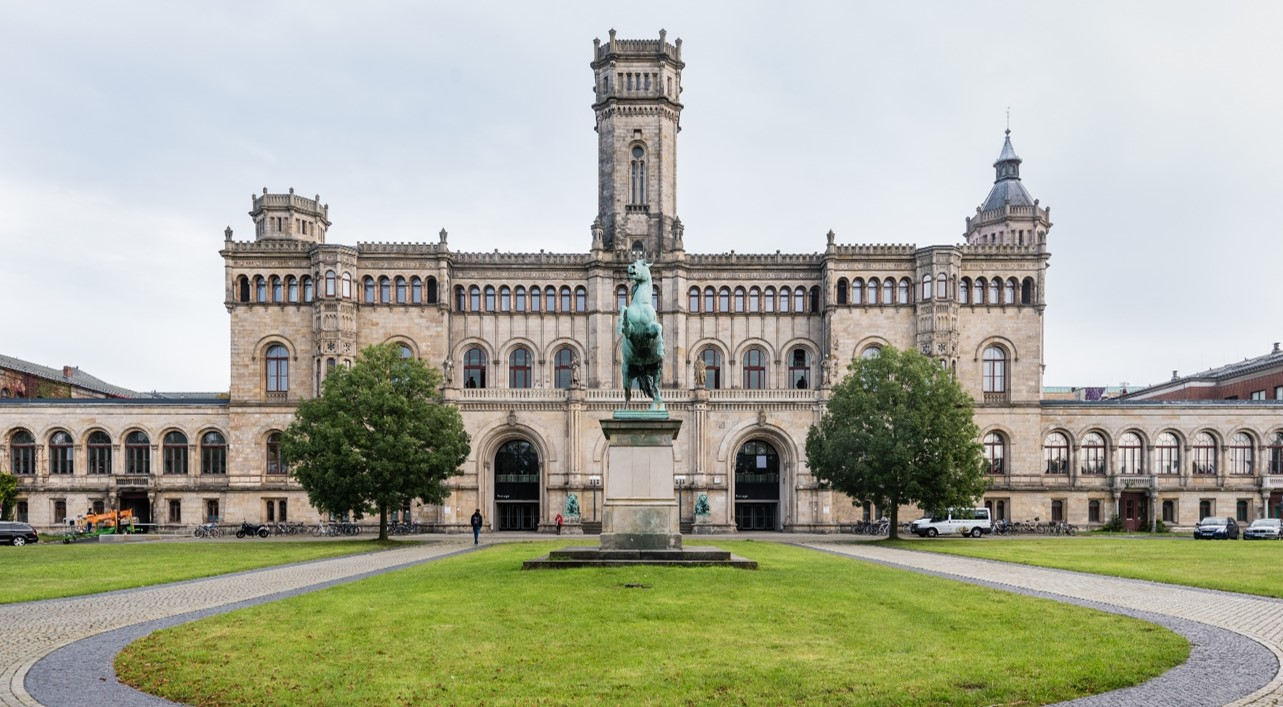
\includegraphics[width=0.65\textwidth]{figures/luh_default_presentation_title_image.jpg}}

% Title page: luhstyle
% \setbeamertemplate{title page}[luhstyle]
% % Add optional title image here
% \addtitlepageimage{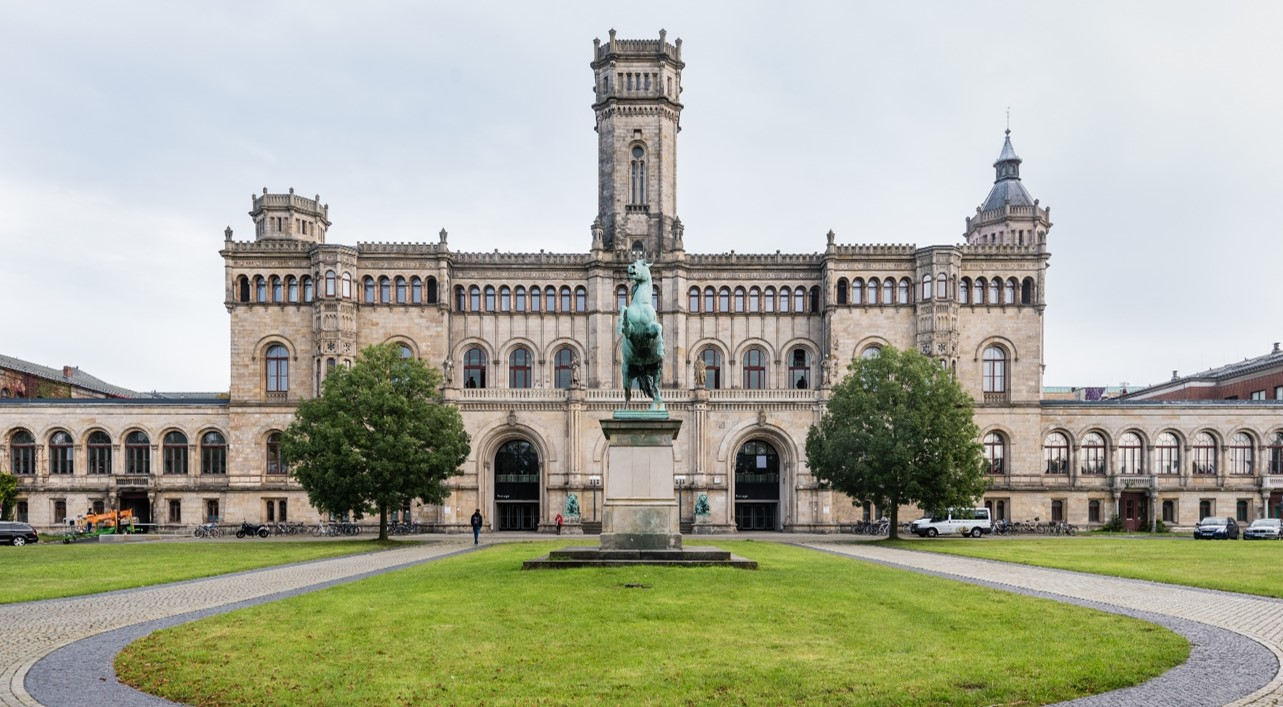
\includegraphics[width=0.75\textwidth]{figures/luh_default_presentation_title_image.jpg}}

\author[Lindauer \& Anand]{Marius Lindauer and Avishek Anand\\[1em]
	
\includegraphics[height=\logoheight]{../latex_main/figures/luh_logo_rgb_0_80_155.pdf}\qquad

\includegraphics[height=\logoheight]{../latex_main/figures/TNT_darkv4}\qquad

\includegraphics[height=\logoheight]{../latex_main/figures/L3S.jpg}	}
\date{Winter Term 2021
}


%%% Custom Packages
%----------------------------------------------------------------------
% Create dummy content
\usepackage{blindtext}

% Adds a frame with the current page layout. Just call \layout inside of a frame.
\usepackage{layout}


\title[Introduction]{iML: Local Explanations}
\subtitle{Motivation}

%\institute{}


\begin{document}
	
	\maketitle

	%-----------------------------------------------------------------------------------------------------------------------------

\begin{frame}[c]{Methodological Motivation}
 
 Explaining the \textbf{local} behavior of a model.
	\begin{itemize}
		\item Some local methods provide insight into the driving factors for a \textbf{particular decision}. 
		\item Others, help to understand the model's decision making in a \textbf{local environment} of the input space.
		\pause
		\smallskip
		\item Local Methods can address questions such as: 
		\begin{itemize}
		    \item \textbf{Why} did the model decide $y$ for input $x$?
		    \item \textbf{How} decides the model for cases similar to $x$?
		    \item \textbf{What} would the ML model have decided if $x$ differed in $\mathcal{X}$?
		    \item  \textbf{Where} does the model fail?
		\end{itemize}  
	\end{itemize}
\end{frame}

\begin{frame}{Social Motivation for Laypersons}

%All these questions can indeed be relevant for the ML modeler. However, unlike in global methods that require expert ML understanding or even domain knowledge, many local methods aim to provide explanations also for laypersons. 
	\begin{itemize}
		\item Explanations for laypersons must be tailored for the \textbf{explainee} (i.e. the person receiving the explanation).
		\pause\smallskip
		\item Thus, such explanations should be case specific, easy for humans to understand, and faithful to the explained mechanism.
		\pause\smallskip
		\item In particular if algorithms make decisions in \textbf{socially/safety critical domains}, end users have justified interest in receiving explanations.
		\pause\smallskip
		\item Local Explanations can not only increase \textbf{user trust}, but also help to detect \textbf{critical local biases} in algorithmic decision making.
		\pause\smallskip
		\item European citizens have the legally binding \textbf{right to explanation} as given in the General Data Protection Regulation (GDPR; DSGVO in Germany).

	\end{itemize}
\end{frame}


% \begin{frame}{GDPR: The Right to Explanation}
%     ``The data subject should have the right not to be subject to a decision, which may include a measure, evaluating personal aspects relating to him or her which is based solely on automated processing and which produces legal effects concerning him or her or similarly significantly affects him or her, such as automatic refusal of an online credit application or e-recruiting practices without any human intervention.
% $\cdots$
% In any case, such processing should be subject to suitable safeguards, which should include specific information to the data subject and the \textbf{right} to obtain human intervention, to express his or her point of view, \textbf{to obtain an explanation of the decision reached after such assessment and to challenge the decision}.
% '' \\[0.2cm] (\href{https://gdpr-text.com/read/recital-71/}{Recital 71, GDPR})
% \end{frame}


\begin{frame}{Example: Husky or Wolf?}
	\begin{itemize}
		\item We trained a model to predict if an image shows a wolf or a husky. 
		\item Below the predictions on six test images are given. 
		\item Do you trust our predictor? 
	\end{itemize}
	\begin{center}
		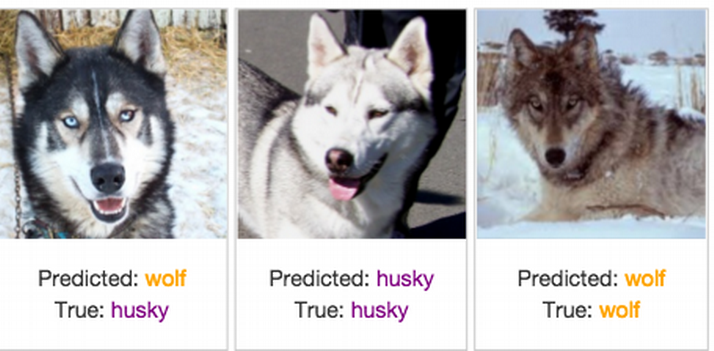
\includegraphics[width=0.3\textwidth]{figure/lime-wolfhusky.png}\\
		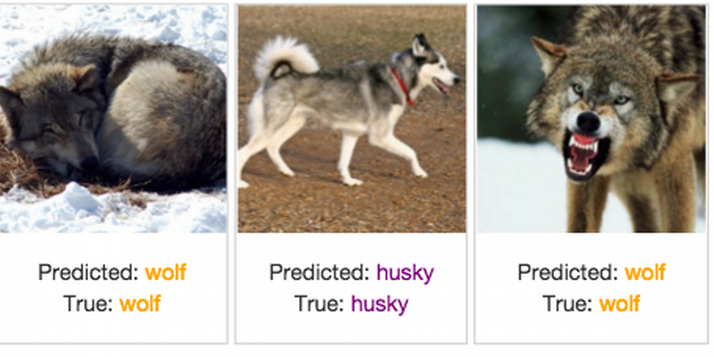
\includegraphics[width=0.3\textwidth]{figure/lime-wolfhusky2.png}\\
		{Source: \lit{Sameer Singh. 2018}{http://www.facweb.iitkgp.ac.in/~niloy/COURSE/Spring2018/IntelligentSystem/PPT_2018/why_should_i_trust_ppt.pdf}}
	\end{center}

\end{frame}
%---------------------------------------------------------------------
\begin{frame}{Example: Husky or Wolf?}
	
	\begin{itemize}
		\item We can use local explanations (in this case LIME) to highlight the parts of an image\\ which led to the prediction.
		\item We can see that our predictor is actually a snow detector. 
	\end{itemize}
	\begin{center}
		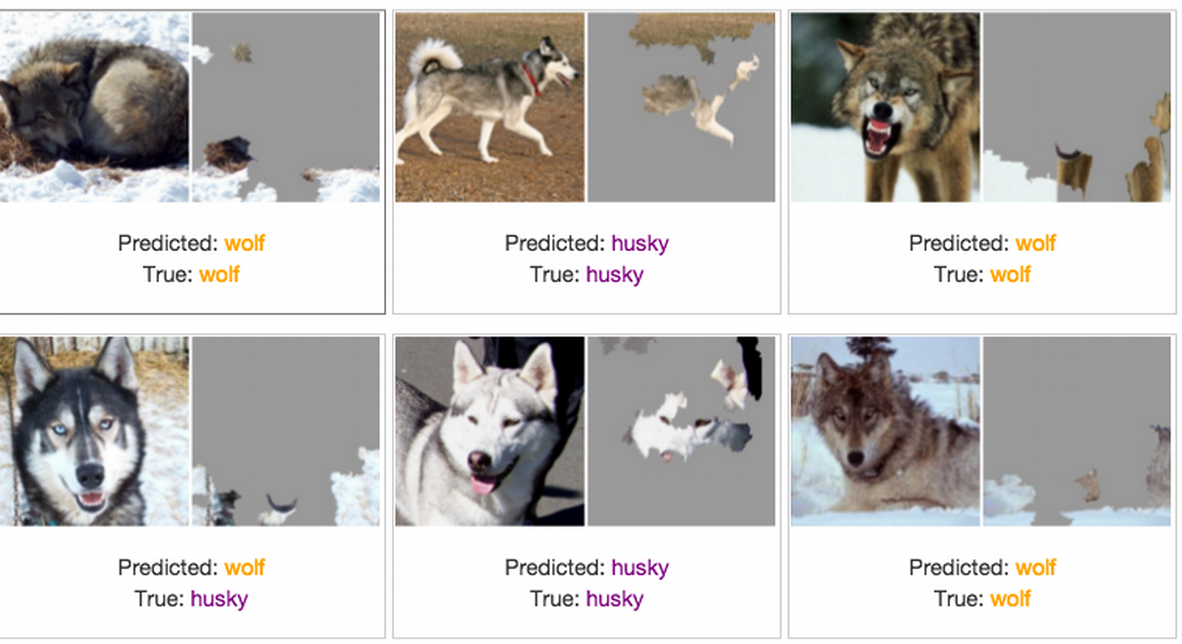
\includegraphics[width=0.5\textwidth]{figure/lime-wolfhusky3.png}\\
		{ Source: \lit{Sameer Singh. 2018}{http://www.facweb.iitkgp.ac.in/~niloy/COURSE/Spring2018/IntelligentSystem/PPT_2018/why_should_i_trust_ppt.pdf}}
	\end{center}
\end{frame}

\begin{frame}{Example: Loan Application}
Assume you are applying at a bank's online portal for a loan and your application gets immediately rejected without reasons.
	\begin{center}
		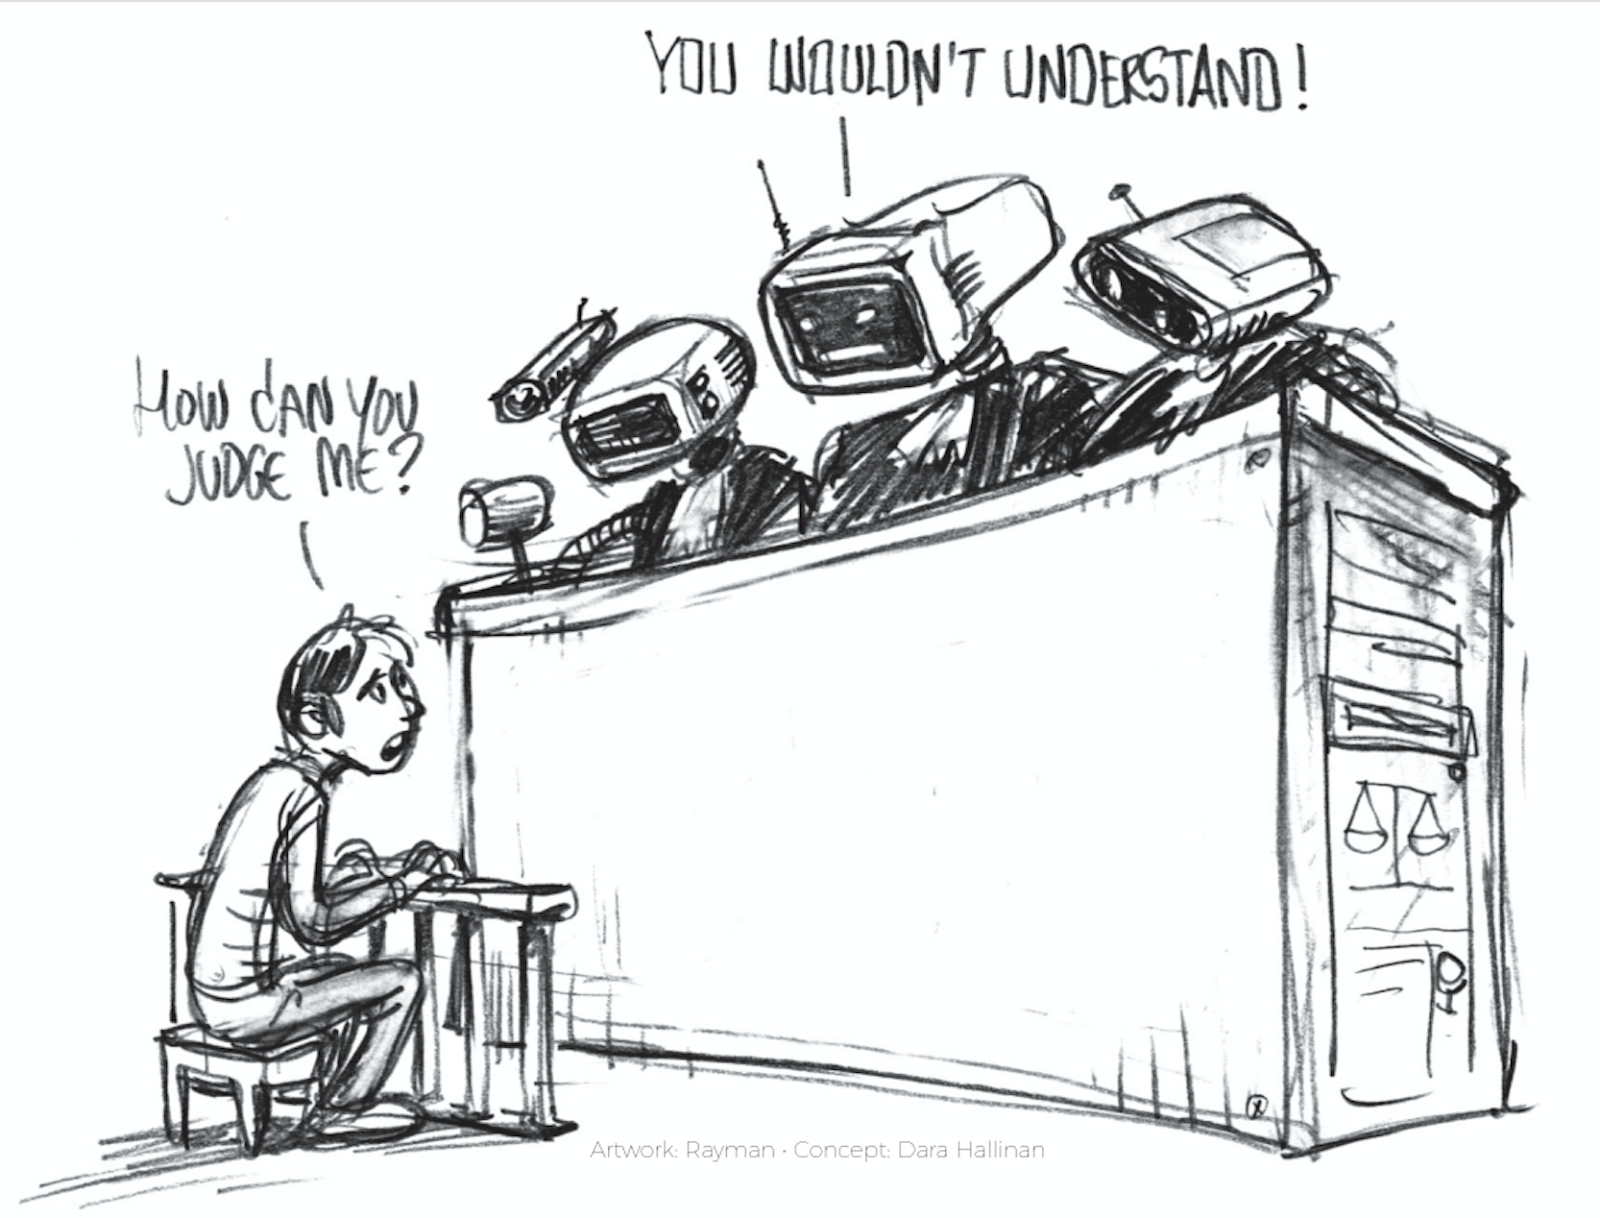
\includegraphics[width=0.3\textwidth]{figure/IntroJudge.png}\\
		{\tiny \textbf{Source:} \href{https://www.elte.hu/content/trendfordulo-az-mi-fejlesztesekben.t.19025}{https://www.elte.hu}}
	\end{center}
	If the bank would use local explanation methods, it could e.g. provide a counterfactual explanation:\\
	``If you were older than 21, your loan application would have been accepted."
\end{frame}

\begin{frame}{Example: Stop or Right-of-Way?}
Assume you work in a car company and are about to use an image classifier for autonomous driving. Then, you show your model the following image (an adversarial example). The classifier is $99\%$ sure it describes a right-of-way sign.
	\begin{center}
		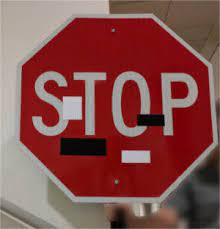
\includegraphics[width=0.22\textwidth]{figure/IntroStop.jpg}\\
		{Source: \lit{Eykholt et. al. 2018}{https://arxiv.org/abs/1707.08945}}
	\end{center}
	Would you entrust other peoples lives into the hands of this software?
\end{frame}

\begin{frame}[c]{Characteristics}
	\begin{itemize}
		\item \textbf{Explanation scope:} Specific prediction, local environment.
		\pause\smallskip
		\item \textbf{Model classes:} Mostly model-agnostic in definition but model-specific for computational reasons, very popular also for deep learning models.
		\pause\smallskip
		\item \textbf{Audience:} ML modelers and laypersons.
		\pause\smallskip
		\item \textbf{Data types:} Many, including tabular, image, text and audio data.
		\pause\smallskip
		\item \textbf{Methods:} Many, most prominent are counterfactual explanations, Shapley values, local interpretable model-agnostic explanations (LIME), adversarial examples, single ICE curve, anchors.
		\pause\smallskip
		\item \textbf{Special:} Due to audience, strong interactions with social sciences. Also, strong connections to cognitive science and neurosciences due to data types.
	\end{itemize}
\end{frame}


\begin{frame}{Credit Dataset}
    \vspace{-2em}
	\begin{itemize}
		\item In this section, we demonstrate local explanation methods on the German credit classification dataset from Kaggle. \href{https://www.kaggle.com/uciml/german-credit}{\beamergotobutton{Click here}}
		\item The dataset has 522 observations and nine features wrt credit and customer information.
		\item The binary target indicates whether a customer has a `good' or `bad' credit risk.  
		\item We combined categories with few case numbers. 
	\end{itemize}
		\begin{center}
			\footnotesize
			\begin{tabular}{ccc}
				\toprule
				name & type & range\\
				\midrule
				age & numeric & [19, 75]\\
				sex & factor & \{male, female\}\\
				job & factor & \{0, 1, 2, 3\}\\
				housing & factor & \{free, own, rent\}\\
				saving.accounts & factor & \{little, moderate, rich\}\\
				checking.accounts & factor & \{little, moderate, rich\}\\
				credit.amount & numeric & [276, 18424]\\
				duration & numeric &  [6, 72]\\
				purpose & numeric &  \{others, car, furniture, radio/TV\}\\
				risk & factor & \{good, bad\}
				\bottomrule
			\end{tabular}
		\end{center}
\end{frame}

\end{document}